\documentclass[usenames,dvipsnames]{beamer}

\usepackage{xcolor}
\usepackage{mathtools}
\usepackage{amsmath,stmaryrd}
\usepackage{tikz}
\usepackage{pgfplots}
\usetikzlibrary{
  calc,
  positioning,
  arrows,
  decorations.markings,
  shapes,
  fit
}
\tikzset{>=latex}
\pgfplotsset{compat=1.14}

% --------------------------------------------------------- x'ed out arrow
\newcommand*{\StrikeThruDistance}{0.2cm}%
\newcommand*{\StrikeThru}{\StrikeThruDistance,\StrikeThruDistance}%
\tikzset{
  strike thru arrow/.style={
    decoration={
      markings, mark=at position 0.5 with {
        \draw [red, very thick, solid,-] ++ (-\StrikeThruDistance,-\StrikeThruDistance) -- ( \StrikeThruDistance, \StrikeThruDistance);
        \draw [red, very thick, solid,-] ++ (-\StrikeThruDistance,\StrikeThruDistance) -- (\StrikeThruDistance, -\StrikeThruDistance);
      }
    },
    postaction={decorate},
  }
}

% --------------------------------------------------------- abbrev
\newcommand{\goedel}[1]{\langle #1 \rangle}
\newcommand{\nats}{\mathbb{N}}
\newcommand{\reals}{\mathbb{R}}
\newcommand{\ints}{\mathbb{Z}}

\newcommand{\setup}{\textbf{SETUP} }
\newcommand{\asign}{\textbf{ASIGN} }
\newcommand{\averify}{\textbf{AVERIFY} }
\newcommand{\verify}{\textbf{VERIFY} }
\newcommand{\keygen}{\textbf{KGEN} }

\newcommand{\mespace}{\mathcal{M}}
\newcommand{\sspace}{\mathcal{S}}
\newcommand{\uspace}{\mathcal{U}}
\newcommand{\kspace}{\mathcal{K}}
\newcommand{\kfspace}{\mathcal{F}}


% --------------------------------------------------------- beamer/document setup
\mode<presentation>

\title{Concurrent Signatures}
% \subtitle{subtitle}

\author{Samir Benzammour}
\date{24th March 2020}
 
\institute[RWTH]{
  Algorithms and Computational Complexity\\
  RWTH Aachen University
}

% fonts etc
\usetheme{Madrid}
\usecolortheme{default}
\usefonttheme{professionalfonts}
\setbeamertemplate{navigation symbols}{}

\AtBeginSection[]
{
  \begin{frame}
    \frametitle{Outline}
    \tableofcontents[currentsection]
  \end{frame}
}

\begin{document}

\frame{\titlepage}

% --------------------------------------------------------- Global
\begin{frame}
	\frametitle{Outline}
	\tableofcontents
\end{frame}

% --------------------------------------------------------- Introduction
\section{Introduction}
\begin{frame}
	\frametitle{Security Model}

	\begin{itemize}
		\item Security is formalized through different key aspects.
		\item e.g. in Ring Signatures one property is \textcolor{red}{xyz}
	\end{itemize}

	And why are they important for our signature scheme?\\
	~\\
	Parallel to this, present an example to illustrate the different key points (maybe using secondary beamer for this)
\end{frame}

\subsection{Concurrent Approach}
\begin{frame}
	\frametitle{Concurrent Approach}
	
	\begin{itemize}
		\setlength\itemsep{1em}
		\item A and B sign messages $M_A$ and $M_B$ respectively
		\item identity is arbitrary \textcolor{blue}{signature ownership not derivable at this point}
		\item commitment upon release of \textit{keystone k}
		\item 
	\end{itemize}
\end{frame}

% --------------------------------------------------------- Concurrent Signature Protocol
\section{Concurrent Signature Protocol}

  \subsection{Scheme}
  \begin{frame}
	\frametitle{Concurrent Scheme}

	\begin{definition}[Concurrent Signature Scheme]<+->
		A \textbf{concurrent signature scheme} is a digital signature scheme, that holds the following algorithms
		\begin{itemize}
			\item \setup
			\item \asign
			\item \averify
			\item \verify
		\end{itemize}
	\end{definition}

  \begin{block}{Notation}<+->
    Let $k$ denote the \textit{keystone}
	\end{block}
\end{frame}

\begin{frame}
	\frametitle{Algorithms}

  \begin{center}	
		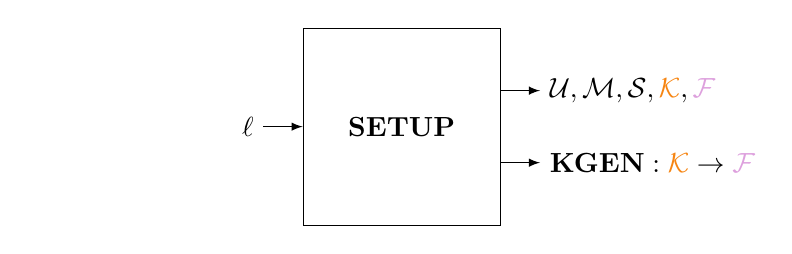
\begin{tikzpicture}
			\visible<1->{\node[draw,minimum size=2.5cm] (setup) {\setup};}

			\visible<2->{\draw[<-] (setup.180) -- ++(180:0.5cm) node [left] {\phantom{$\keygen: \kspace \to \kfspace$}$\ell$};}

      \visible<3->{\draw[->] (setup.20) -- ++(0:0.5cm) node [right] {$\uspace, \mespace, \sspace, \textcolor{BurntOrange}{\kspace}, \textcolor{Plum}{\kfspace}$};}
      \visible<3->{\draw[->] (setup.-20) -- ++(0:0.5cm) node [right] {$\keygen: \textcolor{BurntOrange}{\kspace} \to \textcolor{Plum}{\kfspace}$};}
		\end{tikzpicture}
	\end{center}
\end{frame}

\begin{frame}
	\frametitle{Algorithms}

	\begin{center}	
		\begin{tikzpicture}
			\visible<1->{\node[draw,minimum size=2.5cm] (asign) {\asign};}

			\visible<2->{\draw[<-] (asign.140) -- ++(180:0.5cm) node [left] {\phantom{$\sigma=\goedel{s, h_1, f}$}$\textcolor{MidnightBlue}{X_i}$};}
			\visible<2->{\draw[<-] (asign.180) -- ++(180:0.5cm) node [left] {$\textcolor{MidnightBlue}{X_j}$};}
			\visible<3->{\draw[<-] (asign.220) -- ++(180:0.5cm) node [left] {$x_i$};}
			\visible<4->{\draw[<-] (asign.north) -- ++(90:0.5cm) node [above] {$M$};}
			\visible<5->{\draw[<-] (asign.south) -- ++(-90:0.5cm) node [below] {$f$};}

			\visible<6->{\draw[->] (asign.east) -- ++(0:0.5cm) node [right] {$\sigma = \goedel{s, h_1, f}$};}
		\end{tikzpicture}
	\end{center}

	% \textcolor{blue}{\small introduce everything slide-by-slide}
\end{frame}

\begin{frame}
	\frametitle{Algorithms}

	\begin{center}	
		\begin{tikzpicture}
			\visible<1->{\node[draw,minimum size=2.5cm] (asign) {\averify};}

			\visible<2->{\draw[<-] (asign.140) -- ++(180:0.5cm) node (X_i) [left] {$\textcolor<6>{ForestGreen}{\textcolor<1-5>{MidnightBlue}{X_i}}$};}
			\visible<2->{\draw[<-] (asign.180) -- ++(180:0.5cm) node [left] {$\textcolor<6>{ForestGreen}{\textcolor<1-5>{MidnightBlue}{X_j}}$};}
			\visible<3->{\draw[<-] (asign.220) -- ++(180:0.5cm) node [left] (sigma) {$\textcolor<6>{ForestGreen}{\sigma = \goedel{s, h_1, f}}$};}
			\visible<4->{\draw[<-] (asign.north) -- ++(90:0.5cm) node [above] (message) {$\textcolor<6>{ForestGreen}{M}$};}

			\visible<6->{\node[above left=1cm of X_i, draw, ellipse, dotted, color=ForestGreen, thick] (S) {$\textcolor{ForestGreen}{S}$};}


			\visible<5->{\draw[->] (asign.east) -- ++(0:0.5cm) node [right] {$accept/reject$};}

			% \path (message.north) -- (sigma.south) 
			% 	node[midway, sloped, draw, ellipse, dotted, fit=(message.north east)(sigma.west), inner sep=.5pt]{};
		\end{tikzpicture}
	\end{center}

	% \textcolor{blue}{\small mention symmetric property in talk}
\end{frame}

\begin{frame}
	\frametitle{Algorithms}

	\begin{center}
		\resizebox{.9\hsize}{!}{
			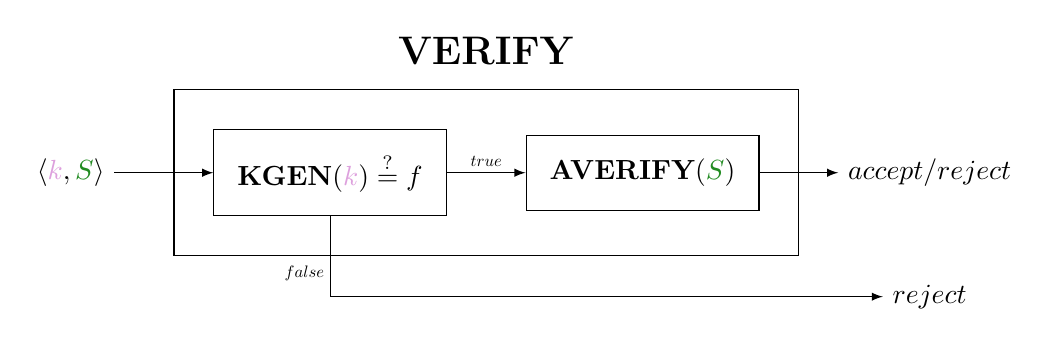
\begin{tikzpicture}[custom/.style = {rectangle, draw, align=center, inner xsep=3mm, inner ysep=3mm}, -latex]
				% nodes
				\visible<3->{\node[custom] (kgen) {$\keygen(\textcolor{Plum}{k}) \overset{?}{=} f$};}
				\visible<5->{\node[custom, right=1cm of kgen.east] (averify) {$\averify(\textcolor{ForestGreen}{S})$};
							\draw (kgen.east) -- node[above, scale=0.6]{$true$} (averify.west);}
				\visible<1->{\node[fit={(kgen) (averify)}, draw, outer ysep=2mm, inner xsep=5mm, inner ysep=5mm, label={\Large\verify}] (outer) {};}
				
				\visible<2->{\node[left=.75cm of outer.west] (input) {$\goedel{\textcolor{Plum}{k},\textcolor{ForestGreen}{S}}$};}
				\visible<6->{\node[right=1cm of averify.east] (output1) {$accept/reject$};}
				\visible<4->{\node[below=1cm of output1.south] (output2) {$reject$};
							\draw  (kgen.south) |- node[left, scale=0.6, yshift=.5cm]{$false$} (output2.west);}

				% connections
				\visible<2->{\draw (input.east) to (kgen.west);}
				\visible<6->{\draw (averify.east) to (output1.west);}
			\end{tikzpicture}
		}
	\end{center}
\end{frame}


  \subsection{Protocol}
  \begin{frame}
	\frametitle{Concurrent Signature Protocol}

	\begin{itemize}[<+->]
		\setlength\itemsep{1em}
		\item Describing signature exchange between A(lice) and B(ob)
		\item Initial signer has to generate keystone
		\item Matching signer responds by using the same keystone-fix
		\item both parties \textit{ambiguous} until $k$ released
	\end{itemize}
\end{frame}

\begin{frame}
	\frametitle{Concurrent Signature Protocol}
	
  \begin{center}
    \resizebox{.95\hsize}{!}{
      \begin{tikzpicture}[node distance=2cm,auto,>=stealth']
        \node[] (bob) {B};
        \node[left = of bob] (alice) {A};
        \node[below of=bob, node distance=7cm] (bobground) {};
        \node[below of=alice, node distance=7cm] (aliceground) {};
        
        % vertical lines
        \draw (alice) -- (aliceground);
        \draw (bob) -- (bobground);
      
        % setup
        \node[left, align=left] at ($(alice)!0.1!(aliceground)$) {\setup};
        \node[right, align=right] at ($(bob)!0.1!(bobground)$) {~\setup};
    
        % k keystone + KGEN
        \visible<2->{\node[left, align=left] at ($(alice)!0.225!(aliceground)$) {$k\in\kspace$, $\textcolor{BurntOrange}{f} = \textbf{KGEN}(\textcolor{Plum}{k})$};}
        
        % ASIGN + Arrow
        \visible<3->{\node[left, align=left] at ($(alice)!0.4!(aliceground)$) {$\asign(\textcolor{MidnightBlue}{X_A, X_B}, x_A, \textcolor{BurntOrange}{f}, M_A)$ \\ {\visible<4->{$= \goedel{s_A, h_A, \textcolor{BurntOrange}{f}} \eqqcolon \textcolor<7>{Red}{\sigma_A}$} }};}
        \visible<5->{\draw[->, dashed] ($(alice)!0.4!(aliceground)$) -- node[sloped, above]{$\textcolor<7>{Red}{\sigma_A}$} ($(bob)!0.45!(bobground)$);}
        
        % AVERIFY
        \visible<6->{\node[right, align=center] at ($(bob)!0.45!(bobground)$) {$\averify(\textcolor<7>{Red}{\sigma_A}, \textcolor{MidnightBlue}{X_A, X_B}, M_A)$};}

        % ASIGN + Arrow
        \visible<8->{\node[right, align=left] at ($(bob)!0.6!(bobground)$) {$\asign(\textcolor{MidnightBlue}{X_B, X_A}, x_B, \textcolor{BurntOrange}{f}, M_B)$};}
        \visible<9->{\draw[->, dashed] ($(bob)!0.6!(bobground)$) -- node[sloped, above]{$\sigma_B$} ($(alice)!0.65!(aliceground)$);}

        % AVERIFY
        \visible<10->{\node[left, align=left] at ($(alice)!0.65!(aliceground)$) {$\averify(\sigma_B, \textcolor{MidnightBlue}{X_B, X_A}, M_B)$};}

        % keystone
        \visible<11->{\draw[->, dashed] ($(alice)!0.8!(aliceground)$) -- node[above]{$\textcolor{Plum}{k}$} ($(bob)!0.85!(bobground)$);}
      \end{tikzpicture}
    }
	\end{center}
\end{frame}

% --------------------------------------------------------- Security Model
\section{Security Model}
\begin{frame}
	\frametitle{Security Model}

	\begin{itemize}
		\item Security is formalized through different key aspects.
		\item e.g. in Ring Signatures one property is \textcolor{red}{xyz}
	\end{itemize}

	And why are they important for our signature scheme?\\
	~\\
	Parallel to this, present an example to illustrate the different key points (maybe using secondary beamer for this)
\end{frame}

  \subsection{Fairness}
  \begin{frame}
	\frametitle{Fairness}

	\begin{itemize}[<+->]
    \setlength\itemsep{1em}
    \item adversary $E$ can query everything except \averify and \verify queries
		\item $E$ returns keystone $k$ and a \textcolor{BurntOrange}{valid} signature $S = \goedel{\sigma, X_c, X_d, M}$
		\item adversary wins if one of the following holds
      \begin{enumerate}[(1.)]
        \setlength\itemsep{.75em}  
				\item $E$ created $k$ s.t. signature is accepted by \verify
				\item $E$ creates additional \textcolor{BurntOrange}{valid} signature $S'$ with same keystone-fix
          \begin{itemize}
            \item but only one of both is accepted by \verify
            \item i.e. $E$ creates signature with same keystone but is not bound by it
          \end{itemize}
			\end{enumerate}
	\end{itemize}
\end{frame}

  \subsection{Ambiguity}
  \begin{frame}
	\frametitle{Ambiguity}

  	
  \begin{center}
    \resizebox{.95\hsize}{!}{
      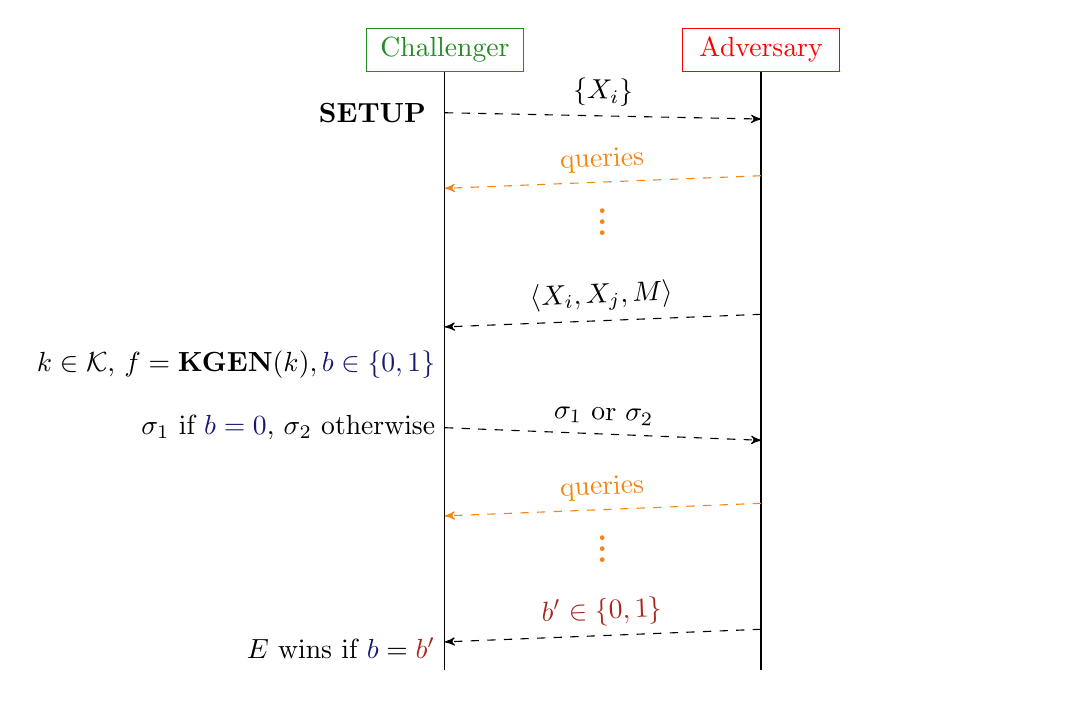
\begin{tikzpicture}[node distance=2cm,auto,>=stealth']
        \node[draw, minimum width = 2cm, color=Red] (adversary) {Adversary};
        \node[draw, minimum width = 2cm, color=ForestGreen, left = of adversary] (challenger) {Challenger};
        \node[below of=adversary, node distance=8cm] (adversaryground) {};
        \node[below of=challenger, node distance=8cm] (challengerground) {};
        
        % vertical lines
        \draw (challenger) -- (challengerground);
        \draw (adversary) -- (adversaryground);
      
        % setup
        \node[left, align=left] at ($(challenger)!0.1!(challengerground)$) {\setup};
        \visible<2->{\draw[->, dashed] ($(challenger)!0.1!(challengerground)$) -- node[sloped, above]{$\{X_i\}$} ($(adversary)!0.11!(adversaryground)$);}
        
        \visible<3->{\draw[->, dashed, BurntOrange] ($(adversary)!0.2!(adversaryground)$) -- node[sloped, above] (queries0) {queries} ($(challenger)!0.22!(challengerground)$);}
        \visible<3->{\node[below = 0mm of queries0, black] {\huge \textcolor{BurntOrange}{$\vdots$}};}

        \visible<4->{\draw[->, dashed] ($(adversary)!0.42!(adversaryground)$) -- node[sloped, above]{$\goedel{X_i, X_j, M}$} ($(challenger)!0.44!(challengerground)$);}

        \visible<5->{\node[left, align=left] at ($(challenger)!0.5!(challengerground)$) {$k\in\kspace$, $f = \textbf{KGEN}(k), \textcolor{MidnightBlue}{b\in\{0,1\}}$};}
        \visible<6->{\node[left, align=left] at ($(challenger)!0.6!(challengerground)$) {$\sigma_1$ if $\textcolor{MidnightBlue}{b=0}$, $\sigma_2$ otherwise};}

        \visible<7->{\draw[->, dashed] ($(challenger)!0.6!(challengerground)$) -- node[sloped, above]{$\sigma_1$ or $\sigma_2$} ($(adversary)!0.62!(adversaryground)$);}

        \visible<8->{\draw[->, dashed, BurntOrange] ($(adversary)!0.72!(adversaryground)$) -- node[sloped, above] (queries1) {queries} ($(challenger)!0.74!(challengerground)$);}
        \visible<8->{\node[below = 0mm of queries1, black] {\huge \textcolor{BurntOrange}{$\vdots$}};}

        \visible<9->{\draw[->, dashed] ($(adversary)!0.92!(adversaryground)$) -- node[sloped, above]{\textcolor{Mahogany}{$b'\in\{0,1\}$}} ($(challenger)!0.94!(challengerground)$);}
        
        \visible<10->{\node[left, align=left] at ($(challenger)!0.95!(challengerground)$) {$E$ wins if $\textcolor{MidnightBlue}{b}=\textcolor{Mahogany}{b'}$};}

        \node[right, align=center] at ($(adversary)!0.42!(adversaryground)$) {\phantom{{$k\in\kspace$, $f = \textbf{KGEN}(k)$}}};
      \end{tikzpicture}
    }
	\end{center}
\end{frame}

  \subsection{Unforgeability}
  \begin{frame}
	\frametitle{Unforgeability}

	\begin{itemize}
		\item consider adversary $E$ and challenger $C$
		\item $C$ runs \setup
		\item $E$ acquires all public variables, $C$ retains all $x_i$
		\item $E$ can request\\[.2cm]
			$\left.\parbox{.5\textwidth}{%
			\begin{itemize}
				\item \textbf{KGen\ldots}
				\item \textbf{KReveal\ldots}
				\item \textbf{ASign\ldots} 
				\item \textbf{AVerify / Verify\ldots}
				\item \textbf{Private Key Extraction\ldots}
			\end{itemize}%
			}\right\}\text{\ldots Queries from } C$
		\item $E$ wins if \textcolor{blue}{$\averify = accept$} and no Private Key Extraction Query was made
		\end{itemize}
\end{frame}

% --------------------------------------------------------- Proof of Lemmata
\section{Concrete Scheme}
\begin{frame}
	\frametitle{Security Model}

	\begin{itemize}
		\item Security is formalized through different key aspects.
		\item e.g. in Ring Signatures one property is \textcolor{red}{xyz}
	\end{itemize}

	And why are they important for our signature scheme?\\
	~\\
	Parallel to this, present an example to illustrate the different key points (maybe using secondary beamer for this)
\end{frame}

% Preliminaries
\begin{frame}
	\frametitle{Discrete Logarithmic Assumption}

	\begin{definition}[discrete logarithm]
		\begin{itemize}
			\item Group $\mathbb{G}$ given
			\item $b^k$ always defined in $\mathbb{G}$ through $b^k = \underbrace{b\cdot b \cdots b}_{k\text{ times}}$
			\item the \textbf{discrete logarithm} is an integer $k$, such that $b^k = a$
		\end{itemize}
	\end{definition}
	\begin{block}{Notation}
		\begin{itemize}
			\item Let $\mathcal{G}$ be a function generating a group
			\item Let $\mathcal{A}$ be a given algorithm
			\item Let $||\cdot||$ be the bit-length of a given integer
		\end{itemize}
	\end{block}
	\textcolor{red}{include definition of a generator?}
\end{frame}

\begin{frame}
	\frametitle{Discrete Logarithmic Assumption}
	\begin{block}{Discrete-Logarithm Experiment $DLog_{\mathcal{A}, \mathcal{G}}(n)$} % consider this experiment with
		\begin{itemize}
			\item Run $\mathcal{G}(1^n)$ to acquire $(\mathbb{G}, q, g)$ where $\mathbb{G}$ is a group, $q$ is its order (whereas $||q|| = n$) and $g\in \mathbb{G}$ is $\mathbb{G}$'s generator
			\item Choose a random $h\in\mathbb{G}$
			\item $\mathcal{A}$ is given $\mathbb{G}, q, g$ and $h$, and outputs $i\in \mathbb{Z}_p$ \textcolor{red}{define what $\mathbb{Z}_p$ is?}
			\item The result of the experiment is $1$ if $g^i = h$, and $0$ otherwise.
		\end{itemize}
	\end{block}
	\begin{definition}
		We say the \textbf{discrete logarithm problem is hard relative to} $\mathcal{G}$ if for all polynomial-time algorithms $\mathcal{A}$ there exists a negligible function $\textsf{negl}$ such that 
			$$\Pr[DLog_{\mathcal{A}, \mathcal{G}}(n) = 1] \leq \textsf{negl}(n)$$
	\end{definition}
\end{frame}
\begin{frame}
	\frametitle{Random Oracle}

	\begin{block}{Definition (Oracle)}
		An \textbf{oracle} (machine) is an abstract machine that takes an input and generates a solution for it without knowing its inner workings.
	\end{block}
	\begin{block}{Definition (Random Oracle)}
		A \textbf{random oracle} is a oracle, which fulfills the following properties
		\begin{itemize}
			\item returns each \textit{unique} request with a truly random value (chosen from output domain)
			\item repeated requests (always) return the same response
		\end{itemize}
	\end{block}
\end{frame}
\begin{frame}
	\frametitle{Definitions}
\end{frame}
\begin{frame}
	\frametitle{Forking Lemma}
\end{frame}

\begin{frame}
	\frametitle{Unforgeability - Proof}
	
	\textit{Proof Idea:}
	\begin{enumerate}[<+->]
		\item Assumption: hardness of the discrete logarithm
		\item Proof by contraposition: Scheme is forgeable with an non-negligible probability
		\item Create system, that uses the adversary to solve the discrete logarithm problem
	\end{enumerate}
\end{frame}

\begin{frame}
	\frametitle{Proof - Setup}

	\begin{itemize}[<+->]
		\item need signature format $\goedel{r_1, h, r_2}$
		\begin{itemize}
			\item easily deriviable from $\sigma = \goedel{s, h_1, h_2}$
		\end{itemize}
		\item $H_1, H_2$ random oracles
		\item $E$ is forging-adversary
		\item $\mathcal{A}$ is an algorithm that solves the discrete logarithm problem
			\begin{itemize}
				\item simulates random oracles and challenger $C$
				\item input: $\goedel{g, X, p , q}$
				\item goal: find $x\in\ints_q$ s.t. $g^x = X \bmod p$
			\end{itemize}
	\end{itemize}
\end{frame}

\begin{frame}
	\frametitle{Proof - Simulation}

	\begin{center}
		\resizebox{\hsize}{!}{
			\begin{tikzpicture}[custom/.style = {rectangle, draw, align=center, minimum width=1.5cm, inner xsep=3mm, inner ysep=3mm}, -latex]
				% nodes
				\visible<3->{\node[custom] (adversary) {$E$};}
				\visible<4->{\node[above=.75cm of adversary] (adversary_input) {$\goedel{g, p, q}$};}
				\phantom{\node[below=.75cm of adversary, align=center] (forged_signature) {$\sigma = \goedel{s, h_1, f}$, \\ $X_c, X_d, M$};}

				\visible<5->{\node[custom, right=.75cm of adversary_input] (participants) {$\mathcal{U}$};}
				\visible<5->{\node[custom, right=.75cm of participants] (priv_keys) {$x_i$};}
				
				\visible<6->{\node[custom, right=.75cm of adversary] (pub_keys) {$X_i {\visible<7->{= g^{x_i} \bmod p}}$};}
				
				\visible<1->{\node[fit={(adversary_input) (priv_keys) (forged_signature)}, draw, outer ysep=2mm, inner xsep=5mm, inner ysep=5mm, label={\Large$\mathcal{A}$}] (outer_box) {};}
				\visible<2->{\node[left=.5cm of outer_box.west] (input) {$\goedel{g, X, p, q}$};}
				
				% connections
				\visible<2->{\draw (input.east) to (outer_box.west);}
				\visible<4->{\draw (adversary_input.south) to (adversary.north);}
				\visible<8->{\draw (pub_keys.west) to (adversary.east);}
				\phantom{\draw (adversary.south) to (forged_signature.north);}
			\end{tikzpicture}
		}
	\end{center}
\end{frame}

\begin{frame}
	\frametitle{Proof - Simulation}

	\begin{itemize}
		\item $H_1, H_2$\textbf{-Queries}
		\item \textbf{KGen-Queries}
		\item \textbf{KReveal-Queries}
		\item \textbf{ASign-Queries} 
		\item \textbf{Private Key Extraction-Queries}
	\end{itemize}
\end{frame}

\begin{frame}
	\frametitle{Proof - Simulation}

	\begin{center}
		\resizebox{\hsize}{!}{
			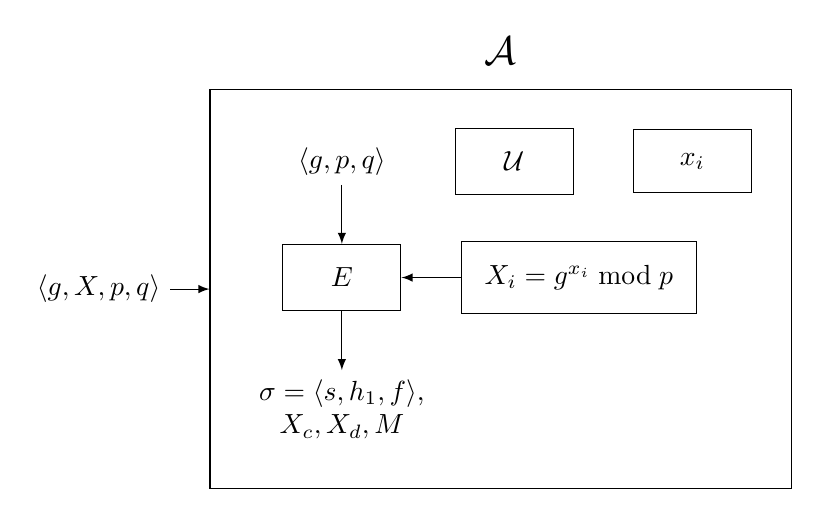
\begin{tikzpicture}[custom/.style = {rectangle, draw, align=center, minimum width=1.5cm, inner xsep=3mm, inner ysep=3mm}, -latex]
				% nodes
				\visible<1->{\node[custom] (adversary) {$E$};}
				\visible<1->{\node[above=.75cm of adversary] (adversary_input) {$\goedel{g, p, q}$};}
				\visible<2->{\node[below=.75cm of adversary, align=center] (forged_signature) {$\sigma = \goedel{s, h_1, f}$, \\ $X_c, X_d, M$};}

				\visible<1->{\node[custom, right=.75cm of adversary_input] (participants) {$\mathcal{U}$};}
				\visible<1->{\node[custom, right=.75cm of participants] (priv_keys) {$x_i$};}
				
				\visible<1->{\node[custom, right=.75cm of adversary] (pub_keys) {$X_i = g^{x_i} \bmod p$};}
				
				\visible<1->{\node[fit={(adversary_input) (priv_keys) (forged_signature)}, draw, outer ysep=2mm, inner xsep=5mm, inner ysep=5mm, label={\Large$\mathcal{A}$}] (outer_box) {};}
				\visible<1->{\node[left=.5cm of outer_box.west] (input) {$\goedel{g, X, p, q}$};}
				
				% connections
				\visible<1->{\draw (input.east) to (outer_box.west);}
				\visible<1->{\draw (adversary_input.south) to (adversary.north);}
				\visible<1->{\draw (pub_keys.west) to (adversary.east);}
				\visible<2->{\draw (adversary.south) to (forged_signature.north);}
			\end{tikzpicture}
		}
	\end{center}
\end{frame}

\begin{frame}
	\frametitle{Proof - Simulation}

	With valid signature, one of the following holds
	\begin{itemize}
		\item No \asign query with $\goedel{X_c, X_d, f, M}$, and no \textbf{Private Key Extraction} query for $X_c$ or $X_d$ 
		\item No \asign query with $\goedel{X_c, X_i, f, M}$, no \textbf{Private Key Extraction} query for $X_c$, and
			\begin{itemize}
				\item $f$ output from previous \keygen query or
				\item $E$ produces keystone $k$ such that $f = \keygen(k)$
			\end{itemize}
	\end{itemize}
\end{frame}

\begin{frame}
	\frametitle{Proof - Simulation}

	\begin{itemize}
		\item if $X_c \neq X_\alpha$, $\mathcal{A}$ aborts because it's lost
		\item Therefore assume: $X_c = X_\alpha = X$
		\item with second case we have:
			$$h = h_1 + f = H_2(g^s X_{c}^{h_1} X_d^f \bmod p ~\|~ M)$$
	\end{itemize}
\end{frame}

\begin{frame}
	\frametitle{Proof - Simulation}

	\textbf{Case 1:} $h = h_1 + f$ never appeared in previous signature query
	\begin{itemize}[<+->]
		\item force $E$ to rerun simulation to produce $(r_1, h', r_2')$ with $h \neq h'$
		\item we have $h = h_1 + f \neq h_1' + f' = h'$
			\begin{itemize}[<+->]
				\item $h_1 \overset{?}{=} h_1'$
				\item \textcolor<+->{BurntOrange}{$f \overset{?}{=} f'$}
			\end{itemize}
		\item due to different output from oracle queries:
			\visible<+->{\begin{equation*}
				% \textcolor<8->{ForestGreen}{g}^s \textcolor<8->{ForestGreen}{X}^{h_1} \textcolor<8->{ForestGreen}{X_d}^{\textcolor<+->{BurntOrange}{f}} = \textcolor<8->{ForestGreen}{g}^{s'} \textcolor<8->{ForestGreen}{X}^{h_1'} \textcolor<8->{ForestGreen}{X_d}^{\textcolor<+->{BurntOrange}{f}}
				g^s X^{\textcolor<8->{BurntOrange}{h_1}} X_d^{\textcolor<8->{BurntOrange}{f}} = g^{s'} X^{\textcolor<8->{BurntOrange}{h_1'}} X_d^{\textcolor<8->{BurntOrange}{f}}
			\end{equation*}}
	\end{itemize}
\end{frame}

\begin{frame}
	\frametitle{Proof - Simulation}

	\begin{align*}
		\visible<1->{\textcolor<2>{ForestGreen}{g}^{\textcolor<3>{BurntOrange}{s}} \textcolor<2>{ForestGreen}{X}^{\textcolor<3>{BurntOrange}{h_1}} \textcolor<2>{ForestGreen}{X_d}^f &= \textcolor<2>{ForestGreen}{g}^{\textcolor<3>{BurntOrange}{s'}} \textcolor<2>{ForestGreen}{X}^{\textcolor<3>{BurntOrange}{h_1'}} \textcolor<2>{ForestGreen}{X_d}^{\textcolor<3>{BurntOrange}{f}} \\}
		\visible<3->{\textcolor<3>{BurntOrange}{s} + x \textcolor<3>{BurntOrange}{h_1} + \textcolor<3>{BurntOrange}{f} &= \textcolor<3>{BurntOrange}{s'} + x \textcolor<3>{BurntOrange}{h_1'} + \textcolor<3>{BurntOrange}{f} \\}
		\visible<4->{s + x h_1 &= s' + x h_1' \\}
		\visible<5->{x &= \frac{s-s'}{h_1' - h_1} \\}
	\end{align*}
	
	\begin{itemize}
		\item<6-> solved the discrete logarithm problem with non-negligible probability
		\item<7-> Henceforth, $\mathcal{A}$ solves the discrete logarithm problem in case 1
	\end{itemize}
\end{frame}

\begin{frame}
	\frametitle{Proof - Simulation}

  \visible<+->{\textbf{Case 2:} $h' = h$, output of signature query $\goedel{X_{c'}, X_{d'}, f', M'}$}

  \begin{itemize}[<+->]
    \item then we have: $\sigma = \goedel{s', h', f'}$
    \item due to $h = h'$ we have
      \[ h = H_2(\textcolor<4->{BurntOrange}{g^s X^{h_1} X_d^f} ~\|~ \textcolor<5->{ForestGreen}{M}) = H_2(\textcolor<4->{BurntOrange}{g^{s'} X_{c'}^{h_1'} X_{d'}^{f'}} ~\|~ \textcolor<5->{ForestGreen}{M'}) = h' \]
    \item<6-> when $X \neq X_{c'}, X_{d'}$ or $X_{c'}, X_{d'} = 0$ but exponents are different
      \[ g^s X^{h_1} X_d^f = X_{c'}^{h_1'} X_{d'}^{f'} \]
      is easily solveable for $x$
  \end{itemize}

\end{frame}

\begin{frame}
  \frametitle{Proof - Simulation}
  
  \begin{itemize}[<+->]
    \item case where $X_{c'},X_{d'} = X$ and exponents are the same is negligible
    \begin{itemize}[<+->]
      \item $X_{c'}$ because no $\asign$ query can be done on $\goedel{X_c, X_i, f, M}$
      \item $X_{d'}$ because some $H_1$ has to match $h_1'$ 
    \end{itemize}
    \item $\mathcal{A}$ can solve the discrete logarithm in case 2
    \item Hence, $\mathcal{A}$ can solve the discrete logarithm $\lightning$
  \end{itemize}

\end{frame}
% --------------------------------------------------------- Conclusion
\section{Conclusion}
To conclude, in this paper we illustrated the concept of concurrent signatures defined by Chen et al., and provided a rundown of the unforgeability proof provided in \cite{chen2004concurrent}.

In short, the concurrent signature scheme enables parties to sign a contract ambiguously, in respect to their own identity, until another piece of information is released.
This piece of information is called the keystone and is generated by one of the participating parties.
To add, the generation of the keystone by one of the participating parties is also the reason why the concurrent signature scheme does not solve the problem with the \textit{truly fair} signature exchange.
However, the presented solution is an adequate enough solution for most applications.

Lastly, keep in mind that the unforgeability property is not a sufficient condition for the security of this scheme.
To see how the other two properties are proven, reference \cite{chen2004concurrent}, or if you are interested on how this scheme is making use of its underlying signature structure, see \cite{abe20021} and \cite{schnorr1991efficient}.

\end{document}